\documentclass[11pt]{article}
\usepackage[margin = 1in]{geometry}
\usepackage{amsmath}
\usepackage{amssymb}
\usepackage{amsthm}
\usepackage{mathtools}
\usepackage{graphicx}
\usepackage{enumitem}
\usepackage{url}
\usepackage[parfill]{parskip}
\usepackage{listings}
\usepackage{caption}
\usepackage{subcaption}
\usepackage[utf8]{inputenc}
\usepackage{xcolor}
\definecolor{codegreen}{rgb}{0,0.6,0}
\definecolor{codegray}{rgb}{0.5,0.5,0.5}
\definecolor{codepurple}{rgb}{0.58,0,0.82}
\definecolor{backcolour}{rgb}{0.95,0.95,0.92}
\lstdefinestyle{mystyle}{
	backgroundcolor=\color{backcolour},   
	commentstyle=\color{codegreen},
	keywordstyle=\color{magenta},
	numberstyle=\tiny\color{codegray},
	stringstyle=\color{codepurple},
	basicstyle=\ttfamily\footnotesize,
	breakatwhitespace=false,         
	breaklines=true,                 
	captionpos=b,                    
	keepspaces=true,                 
	numbers=left,                    
	numbersep=5pt,                  
	showspaces=false,                
	showstringspaces=false,
	showtabs=false,                  
	tabsize=2
}
\lstset{style=mystyle}
\newcommand{\skipline}{\vspace{\baselineskip}}
\newcommand{\spacer}{\noalign{\medskip}}
\newcommand{~}{\sim}
\newcommand{\approches}{\rightarrow}
\newcommand{\qarrow}{\quad \rightarrow \quad}
\newcommand{\qqarrow}{\qquad \rightarrow \qquad}
\newcommand{\qqtext}[1]{\qquad \text{ #1 } \qquad}
\newcommand{\pard}[2]{\frac{\partial #1}{\partial #2}}
\newcommand{\answer}[1]{\textbf{\boldmath #1}}
\newenvironment{problem}[1]{\textbf{Problem #1: }}{\newpage}

\begin{document}
	
	\begin{center}
		\textbf{Homework 5} \\
		\textbf{Partial Differential Equations} \\
		\textbf{Math 531} \\
		\textbf{Stephen Giang RedID: 823184070} \\
		\skipline \skipline
	\end{center}

	\begin{problem}{1}
		Consider the function $f(x) = x^2$.Use MatLab to create the computer graphics
		to show the following:

		\begin{itemize}[label=-]
			\item In all graphs include the original function for $x \in [-4, 4]$. (Don’t extend to the full
			interval.)

			\item Find the Fourier sine series, including the Fourier coefficients, for $f(x)$ for $x \in [0,3]$
			\\ \\
			Notice the following Fourier sine series:
			\[f(x) = x^2 = \sum_{n=1}^{\infty} B_n\sin\left(\frac{n\pi x}{3}\right)\]
			Notice the following:
			\begin{align*}
				\int x^2 \sin\left(\frac{n\pi x}{3}\right)\,dx &= \frac{-3x^2}{n\pi}\cos\left(\frac{n\pi x}{3}\right) + \frac{6}{n\pi}\int x\cos\left(\frac{n\pi x}{3}\right)\,dx \\
				&= \frac{-3x^2}{n\pi}\cos\left(\frac{n\pi x}{3}\right) + \frac{18x}{(n\pi)^2}\sin\left(\frac{n\pi x}{3}\right) - \frac{18}{(n\pi)^2}\int \sin\left(\frac{n\pi x}{3}\right)\,dx \\
				&= \frac{-3x^2}{n\pi}\cos\left(\frac{n\pi x}{3}\right) + \frac{18x}{(n\pi)^2}\sin\left(\frac{n\pi x}{3}\right) + \frac{54}{(n\pi)^3} \cos\left(\frac{n\pi x}{3}\right)
			\end{align*}
			Notice the Fourier coefficient:
			\begin{align*}
				B_n &= \frac{2}{3} \int_{0}^{3} x^2 \sin\left(\frac{n\pi x}{3}\right)\,dx \\
				&= \frac{2}{3}\left(\frac{-3x^2}{n\pi}\cos\left(\frac{n\pi x}{3}\right) + \frac{18x}{(n\pi)^2}\sin\left(\frac{n\pi x}{3}\right) + \frac{54}{(n\pi)^3} \cos\left(\frac{n\pi x}{3}\right)\right)\bigg|_0^3 \\
				&=  \frac{-18}{n\pi}\cos\left(n\pi\right) + \frac{36}{(n\pi)^3} \cos\left(n\pi\right) - \frac{36}{(n\pi)^3}
			\end{align*}
			\newpage
			\item Graph the original function and the Fourier sine series, where you use 3, 5, 10, 20,
			and 100 terms. Show the graph for $x \in [-6, 6]$.
			\begin{figure}[h!]
				\centering
				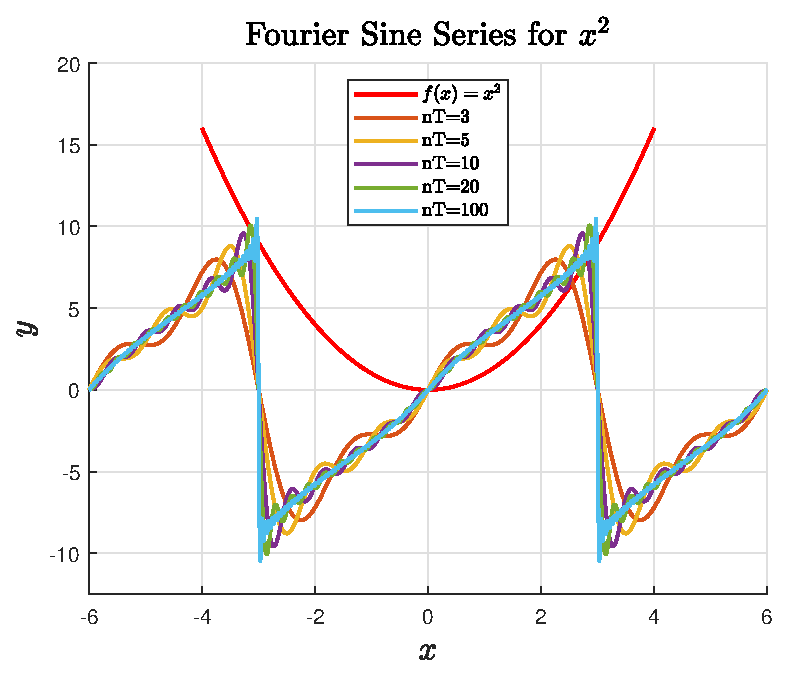
\includegraphics[width=.5\textwidth]{Prob1Sine}
			\end{figure}
			\begin{lstlisting}[language=Matlab]
close all; clc; clear;
figure();hold on; grid on;

x = linspace(-4,4,2000);   
g = x.^2;
plot(x,g,'r-','LineWidth',1.5)

numTerms = [3,5,10,20,100];
x = linspace(-6,6,2000);
for i = 1 : size(numTerms,2)
	plot(x,diffFTerms(numTerms(i), x),'LineWidth',1.5); 
end 

xlabel('$x$','FontSize',16,'interpreter','latex'); 
ylabel('$y$','FontSize',16, 'interpreter','latex');
title('Fourier Sine Series for $x^2$','FontSize',16, 'interpreter','latex');
legend('$f(x) = x^2$','nT=3', 'nT=5', 'nT=10', 'nT=20', 'nT=100', 'interpreter','latex', 'location', 'north' );
xlim([-6,6]);
ylim([-12.5,20]);

print -depsc Prob1Sine.eps

function f = diffFTerms(Nf, x)  
b = zeros(1,Nf); 
f = 0;
	for n = 1 : Nf     
		npi = n * pi;
		b(n) = ( (-18/npi)*cos(npi) ) + ( (36/(npi^3))*cos(npi) ) + ( 36/(npi^3) );    
		fn = b(n)*sin((npi*x)/3);     
		f=f+fn; 
	end
end

			\end{lstlisting}
			\newpage
			\item Find the Fourier cosine series, including the Fourier coefficients, for f(x) for $x \in [0, 3]$.
			\\ \\
			Notice the following Fourier cosine series:
			\[f(x) = x^2 = A_0 + \sum_{n=1}^{\infty} A_n\cos\left(\frac{n\pi x}{3}\right)\]
			Notice the following:
			\begin{align*}
				\int x^2 \cos\left(\frac{n\pi x}{3}\right)\,dx &= \frac{3x^2}{n\pi}\sin\left(\frac{n\pi x}{3}\right) - \frac{6}{n\pi}\int x\sin\left(\frac{n\pi x}{3}\right)\,dx \\
				&= \frac{3x^2}{n\pi}\sin\left(\frac{n\pi x}{3}\right) + \frac{18x}{(n\pi)^2}\cos\left(\frac{n\pi x}{3}\right) - \frac{18}{(n\pi)^2}\int \cos\left(\frac{n\pi x}{3}\right)\,dx \\
				&= \frac{3x^2}{n\pi}\sin\left(\frac{n\pi x}{3}\right) + \frac{18x}{(n\pi)^2}\cos\left(\frac{n\pi x}{3}\right) - \frac{54}{(n\pi)^3} \sin\left(\frac{n\pi x}{3}\right)
			\end{align*}
			Notice the Fourier coefficients:
			\begin{align*}
				A_0 &= \frac{1}{3}\int_{0}^3 x^2\,dx = \frac{x^3}{9} \bigg|_0^3 = 3 \\
				A_n &= \frac{2}{3} \int_{0}^{3} x^2 \cos\left(\frac{n\pi x}{3}\right)\,dx \\
				&= \frac{2}{3}\left(\frac{3x^2}{n\pi}\sin\left(\frac{n\pi x}{3}\right) + \frac{18x}{(n\pi)^2}\cos\left(\frac{n\pi x}{3}\right) - \frac{54}{(n\pi)^3} \sin\left(\frac{n\pi x}{3}\right)\right)\bigg|_0^3 \\
				&= \frac{36}{(n\pi)^2}\cos(n\pi)
			\end{align*}
			\newpage
			\item Graph the original function and the Fourier cosine series, where you use 3, 5, 10,
			and 20 terms. Show the graph for $x \in [-6, 6]$.
			\begin{figure}[h!]
				\centering
				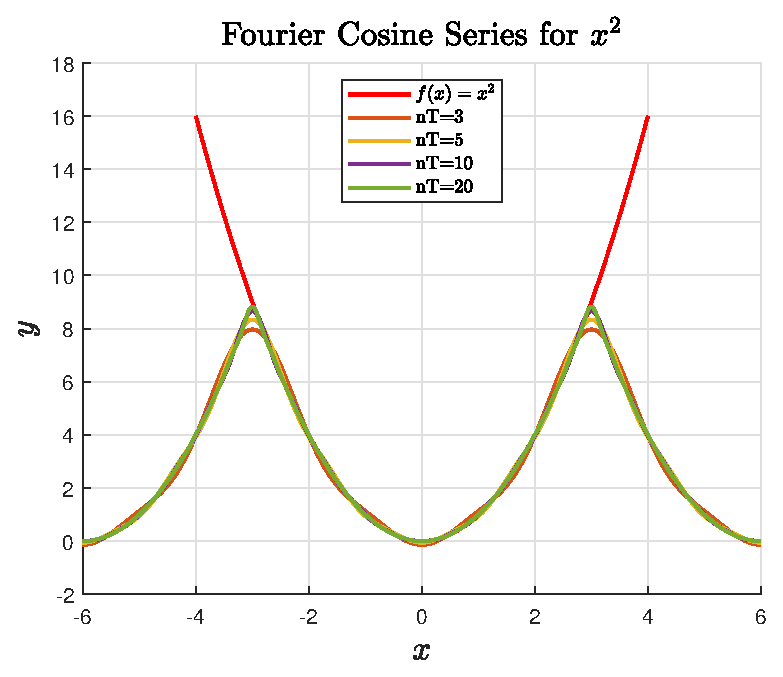
\includegraphics[width=.5\textwidth]{Prob1Cosine}
			\end{figure}
			\begin{lstlisting}[language=Matlab]
close all; clc; clear;
figure();hold on; grid on;

x = linspace(-4,4,2000);   
g = x.^2;
plot(x,g,'r-','LineWidth',1.5)

numTerms = [3,5,10,20];
x = linspace(-6,6,2000);
for i = 1 : size(numTerms,2)
	plot(x,diffFTerms(numTerms(i), x),'LineWidth',1.5); 
end 

xlabel('$x$','FontSize',16,'interpreter','latex'); 
ylabel('$y$','FontSize',16, 'interpreter','latex');
title('Fourier Cosine Series for $x^2$','FontSize',16, 'interpreter','latex');
legend('$f(x) = x^2$','nT=3', 'nT=5', 'nT=10', 'nT=20', 'nT=100', 'interpreter','latex', 'location', 'north' );
xlim([-6,6]);
ylim([-2,18]);

print -depsc Prob1Cosine.eps

function f = diffFTerms(Nf, x) 
a0 = 3;
a = zeros(1,Nf); 
f = a0;
	for n = 1 : Nf     
		npi = n * pi;
		a(n) = (36 / (npi^2))*cos(npi);   
		fn = a(n)*cos((npi*x)/3);     
		f=f+fn; 
	end
end
			\end{lstlisting}
		\end{itemize}
	\end{problem}
	
	% Page 118
	\begin{problem}{2}
		Exercise 3.3.1c:
		\\ \\
		For the following functions, sketch $f(x)$, the Fourier series of $f(x)$, the Fourier sine
		series of $f(x)$, and the Fourier cosine series of $f(x)$:
		\[f(x) = \begin{cases}
			x & x < 0 \\ 1 + x & x > 0 
		\end{cases}\]
		Notice the Fourier Series:
		\begin{align*}
			f(x) &= A_0 + \sum_{n=1}^{\infty} A_n\cos \frac{n\pi x}{L} + \sum_{n=1}^{\infty} B_n\sin \frac{n\pi x}{L} \\
			A_0 &= \frac{1}{2L}\int_{-L}^0 f(x)\,dx + \frac{1}{2L}\int_{0}^L f(x)\,dx =\frac{1}{2L}\int_{-L}^0 x\,dx +  \frac{1}{2L}\int_{0}^L (1 + x)\,dx \\
			&= \frac{x^2}{4L}\bigg|_{-L}^0 +  \left(\frac{x}{2L} + \frac{x^2}{4L}\right) \bigg|_0^L = \frac{1}{2} 
			\\ \\
			A_n &= \frac{1}{L} \int_{-L}^0 f(x)\cos \frac{n\pi x}{L}\,dx + \frac{1}{L} \int_{0}^L f(x)\cos \frac{n\pi x}{L}\,dx = \frac{1}{L} \int_{-L}^0 x\cos \frac{n\pi x}{L}\,dx + \frac{1}{L} \int_{0}^L  (1+x)\cos \frac{n\pi x}{L}\,dx \\
			&= \frac{1}{L} \left(\frac{xL}{n\pi}\sin\frac{n\pi x}{L} + \left(\frac{L}{n\pi}\right)^2\cos\frac{n\pi x}{L}\right)\bigg|_{-L}^0 + \frac{1}{L} \left(\frac{(1+x)L}{n\pi}\sin\frac{n\pi x}{L} + \left(\frac{L}{n\pi}\right)^2\cos\frac{n\pi x}{L}\right)\bigg|_{0}^L \\
			&= \frac{x}{n\pi}\sin\frac{n\pi x}{L} + \left(\frac{L}{(n\pi)^2}\right)\cos\frac{n\pi x}{L}\bigg|_{-L}^0 + \frac{(1+x)}{n\pi}\sin\frac{n\pi x}{L} + \left(\frac{L}{(n\pi)^2}\right)\cos\frac{n\pi x}{L}\bigg|_{0}^L \\
			&= \frac{L}{(n\pi)^2} - \frac{(-1)^nL}{(n\pi)^2} + \frac{(-1)^nL}{(n\pi)^2} - \frac{L}{(n\pi)^2} = 0
			\\ \\
			B_n &= \frac{1}{L} \int_{-L}^0 f(x)\sin \frac{n\pi x}{L}\,dx + \frac{1}{L} \int_{0}^L f(x)\sin \frac{n\pi x}{L}\,dx = \frac{1}{L} \int_{-L}^0 x\sin \frac{n\pi x}{L} + \frac{1}{L} \int_{0}^L (1+x)\sin \frac{n\pi x}{L} \\
			&= \frac{1}{L} \left(\frac{-xL}{n\pi}\cos\frac{n\pi x}{L} + \left(\frac{L}{n\pi}\right)^2\sin\frac{n\pi x}{L}\right)\bigg|_{-L}^0 + \frac{1}{L} \left(\frac{-(1+x)L}{n\pi}\cos\frac{n\pi x}{L} + \left(\frac{L}{n\pi}\right)^2\sin\frac{n\pi x}{L}\right)\bigg|_{0}^L \\
			&= \frac{-x}{n\pi}\cos\frac{n\pi x}{L} + \left(\frac{L}{(n\pi)^2}\right)\sin\frac{n\pi x}{L}\bigg|_{-L}^0 + \frac{-(1+x)}{n\pi}\cos\frac{n\pi x}{L} + \left(\frac{L}{(n\pi)^2}\right)\sin\frac{n\pi x}{L}\bigg|_{0}^L \\
			&= \frac{-L(-1)^n}{n\pi} + \frac{-(1 + L)(-1)^n}{n\pi} = \frac{-(1 + 2L)(-1)^n}{n\pi}
		\end{align*}
		Notice the Fourier sine and cosine series of $f(x)$ respectively:
		\[f(x) ~ \sum_{n=1}^{\infty} \frac{-2L (-1)^n}{(n\pi)^2}\sin \frac{n\pi x}{L} \qquad f(x) ~ 1 + \frac{L}{2} + \sum_{n=1}^{\infty} \frac{2L ((-1)^n - 1)}{(n\pi)^2}\cos \frac{n\pi x}{L} \]
		\begin{figure}[h!]
			\centering
			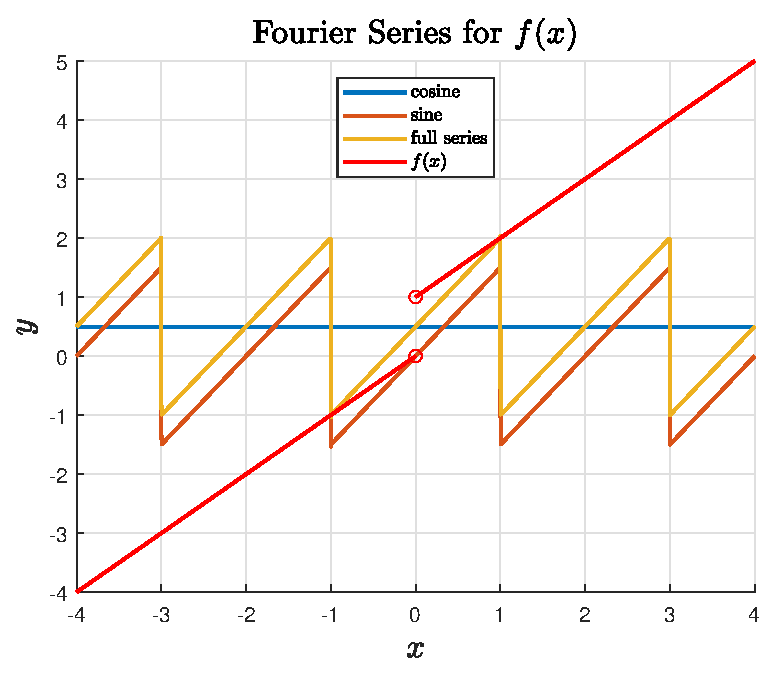
\includegraphics[width=.5\textwidth]{Prob2}
		\end{figure}
		\newpage
		\begin{lstlisting}[language=Matlab]
close all; clc; clear;
figure();hold on; grid on;

L = 1;

x = linspace(-4,4,2000);
for i = 1 : 3
	plot(x,diffFTerms(x, L, i),'LineWidth',1.5);
end

x = linspace(-4,0,2000);   
g = x;
plot(x,g,'r-','LineWidth',1.5)
plot(0,0,'ro')
x = linspace(0,4,2000); 
g = 1+x;
plot(x,g,'r-','LineWidth',1.5)
plot(0,1,'ro')

xlabel('$x$','FontSize',16,'interpreter','latex'); 
ylabel('$y$','FontSize',16, 'interpreter','latex');
title('Fourier Series for $f(x)$','FontSize',16, 'interpreter','latex');
legend('cosine', 'sine', 'full series', '$f(x)$', 'interpreter','latex', 'location', 'north' );

print -depsc Prob2.eps

function f = diffFTerms(x, L, num)
	Nf = 1000;
	a0 = (1/2);
	a = zeros(1,Nf);
	b = zeros(1,Nf);
	if (num == 2), f = 0;
	else, f = a0; 
	end
	for n = 1 : Nf     
		npi = n * pi;
		a(n) = 0; 
		b(n) = (-(1 + (2*L))*((-1)^n)) / (npi);
		if (num == 1), fn = a(n)*cos((npi*x)/L); 
		elseif (num == 2), fn = b(n)*sin((npi*x)/L);
		elseif (num == 3), fn = a(n)*cos((npi*x)/L) + b(n)*sin((npi*x)/L);
		end 
		f=f+fn; 
	end
end			
		\end{lstlisting}
		
	\end{problem}

	\begin{problem}{3}
		Exercise 3.3.14:
		\begin{enumerate}[label = (\alph*)]
			\item Consider a function $f(x)$ that is even around $x = L/2$. Show that the odd coefficients ($n$ odd) of the Fourier cosine series of $f(x)$ on $0 \leq x \leq L$ are zero.
			\\ \\
			Notice the Fourier cosine series of $f(x)$:
			\[A_n = \frac{2}{L}\int_{0}^L f(x)\cos \frac{n\pi x}{L}\,dx\]
			We disregard $A_0$ because we are focusing on odd values of $n$.
			\\ \\
			Notice the following:
			\[\cos \frac{n\pi (L/2)}{L} = \cos \frac{n\pi}{2} = 0 \text{ for } n = 2k + 1 \quad k = 1,3,5...\]
			Notice the following:
			\begin{align*}
				\cos\left(\frac{n\pi(\frac{L}{2} + x)}{L}\right) &= \cos\left(\frac{n\pi(\frac{L}{2})}{L} + \frac{n\pi x}{L}\right) \\
				&= \cos\left(\frac{n\pi(\frac{L}{2})}{L}\right)\cos\left(\frac{n\pi x}{L}\right) - \sin\left(\frac{n\pi(\frac{L}{2})}{L}\right)\sin\left(\frac{n\pi x}{L}\right) \\
				&= -\sin\left(\frac{n\pi(\frac{L}{2})}{L}\right)\sin\left(\frac{n\pi x}{L}\right) \\
				&= -\left(\cos\left(\frac{n\pi(\frac{L}{2})}{L}\right)\cos\left(\frac{n\pi x}{L}\right) + \sin\left(\frac{n\pi(\frac{L}{2})}{L}\right)\sin\left(\frac{n\pi x}{L}\right)\right) \\
				&= -\cos\left(\frac{n\pi(\frac{L}{2})}{L} - \frac{n\pi x}{L}\right) \\
				&= -\cos\left(\frac{n\pi(\frac{L}{2} - x)}{L}\right)
			\end{align*}
			So we get that $\cos \frac{n\pi x}{L}$ is odd about $L/2$ with $n$ being odd as well:
			\\ \\
			Now because $f(x)$ is even about $x = L/2$ and $\cos \frac{n\pi x}{L}$ is odd about $x = L/2$, we get that their product is odd about $x = L/2$, this means we get the following:
			\[\frac{2}{L}\int_{0}^{L/2} f(x)\cos \frac{n\pi x}{L}\,dx = -\frac{2}{L}\int_{L/2}^L f(x)\cos \frac{n\pi x}{L}\,dx \]
			Thus, we get that for $n$ being odd, the coefficients $A_n$ is zero:
			\[A_n = \frac{2}{L}\int_{0}^L f(x)\cos \frac{n\pi x}{L}\,dx = 0\]
			\newpage
			\item Explain the result of part (a) by considering a Fourier cosine series of $f(x)$ on the
			interval $0 \leq x \leq L/2$.
			\\ \\
			Notice the Fourier cosine series of $f(x)$:
			\[A_n = \frac{2}{L/2}\int_{0}^{L/2} f(x)\cos \frac{n\pi x}{L/2}\,dx\]
			We disregard $A_0$ because we are focusing on odd values of $n$.
			\\ \\
			Notice the following:
			\[\cos \frac{n\pi (L/4)}{L/2} = \cos \frac{n\pi}{2} = 0 \text{ for } n = 2k + 1 \quad k = 1,3,5...\]
			Notice the following:
			\begin{align*}
				\cos\left(\frac{n\pi(\frac{L}{4} + x)}{L}\right) &= \cos\left(\frac{n\pi(\frac{L}{4})}{L} + \frac{n\pi x}{L}\right) \\
				&= \cos\left(\frac{n\pi(\frac{L}{4})}{L}\right)\cos\left(\frac{n\pi x}{L}\right) - \sin\left(\frac{n\pi(\frac{L}{4})}{L}\right)\sin\left(\frac{n\pi x}{L}\right) \\
				&= -\sin\left(\frac{n\pi(\frac{L}{4})}{L}\right)\sin\left(\frac{n\pi x}{L}\right) \\
				&= -\left(\cos\left(\frac{n\pi(\frac{L}{4})}{L}\right)\cos\left(\frac{n\pi x}{L}\right) + \sin\left(\frac{n\pi(\frac{L}{4})}{L}\right)\sin\left(\frac{n\pi x}{L}\right)\right) \\
				&= -\cos\left(\frac{n\pi(\frac{L}{4})}{L} - \frac{n\pi x}{L}\right) \\
				&= -\cos\left(\frac{n\pi(\frac{L}{4} - x)}{L}\right)
			\end{align*}
			So we get that $\cos \frac{n\pi x}{L/2}$ is odd about $L/4$ with $n$ being odd as well:
			\\ \\
			Now because $f(x)$ is even about $x = L/2$, that means that $\int_0^L f(x)\,dx = 2\int_{0}^{L/2} f(x)\,dx$ and $\cos \frac{n\pi x}{L/2}$ is odd about $x = L/4$, we get that their product is odd about $x = L/2$, this means we get the following:
			\[\frac{2}{L/2}\int_{0}^{L/4} f(x)\cos \frac{n\pi x}{L/2}\,dx = -\frac{2}{L/2}\int_{L/4}^{L/2} f(x)\cos \frac{n\pi x}{L/2}\,dx \]
			Thus, we get that for $n$ being odd, the coefficients $A_n$ is zero:
			\[A_n = \frac{2}{L/2}\int_{0}^{L/2} f(x)\cos \frac{n\pi x}{L/2}\,dx = 0\]
		\end{enumerate}
	\end{problem}
	% Page 130
	\begin{problem}{4}
		Exercise 3.4.6
		\\ \\
		There are some things wrong in the following demonstration. Find the mistakes and
		correct them.
		\\
		In this exercise we attempt to obtain the Fourier cosine coefficients of $e^x$:
		\[e^x = A_0 + \sum_{n=1}^\infty A_n\cos \frac{n\pi x}{L}. \tag{4.22}\]
		Differentiating yields
		\[e^x = -\sum_{n=1}^\infty \frac{n \pi}{L} A_n\sin \frac{n\pi x}{L},\]
		the Fourier sine series of $e^x$. Differentiating again yields
		\[e^x = -\sum_{n=1}^\infty \left(\frac{n \pi}{L}\right)^2 A_n\cos \frac{n\pi x}{L}. \tag{4.23}\]
		Since Equations (4.22) and (4.23) give the Fourier cosine series of $e^x$, they must be
		identical. Thus,
		\[\begin{rcases*}
			A_0 = 0 \\ A_n = 0
		\end{rcases*} \text{(obviously wrong!).}\]
		By correcting the mistakes, you should be able to obtain $A_0$ and $A_n$ \textit{without} using the
		typical technique, that is, $A_n = 2/L \int_{0}^L e^x\cos n\pi x / L\,dx$.
		\\ \\
		Notice we cannot differentiate $e^x$ Fourier sine Series as it is not continuous:
		\[f(0) = e^0 = 1 \not = -\sum_{n=1}^\infty \frac{n \pi}{L} A_n\sin 0 = 0 \qquad f(L) = e^L \not = -\sum_{n=1}^\infty \frac{n \pi}{L} A_n\sin n\pi = 0\]
		Because we cannot differentiate the Fourier sine Series term by term, we get the following:
		\begin{align*}
			f'(x) &~ \frac{f(L) - f(0)}{L} + \sum_{n=1}^\infty \left(\frac{n\pi}{L}B_n + \frac{2((-1)^nf(L) - f(0))}{L}\right)\cos \frac{n\pi x}{L} \\
			e^x &~ \frac{e^L - 1}{L} + \sum_{n=1}^\infty \left(\frac{n\pi}{L}\left(-\frac{n\pi}{L}A_n\right) + \frac{2((-1)^ne^L - 1)}{L}\right)\cos \frac{n\pi x}{L}
		\end{align*}
		Now we set our result equal to our original Fourier cosine series:
		\[A_0 + \sum_{n=1}^\infty A_n\cos \frac{n\pi x}{L} = \frac{e^L - 1}{L} + \sum_{n=1}^\infty \left(\frac{n\pi}{L}\left(-\frac{n\pi}{L}A_n\right) + \frac{2((-1)^ne^L - 1)}{L}\right)\cos \frac{n\pi x}{L}\]
		Now we get the following results:
		\[A_0 = \frac{e^L - 1}{L} \qquad A_n = -\frac{n^2\pi^2}{L^2}A_n + \frac{2((-1)^ne^L - 1)}{L}  \qarrow A_n = \frac{2L((-1)^ne^L - 1)}{L^2 + n^2\pi^2}\]
	\end{problem}

	\begin{problem}{5}
		Exercise 3.4.11:
		\\ \\
		Consider the \textit{nonhomogeneous} heat equation (with a steady heat source):
		\[\pard{u}{t} = k\pard{^2u}{x^2} + g(x)\]
		Solve this equation with the initial condition
		\[u(x,0) = f(x)\]
		and the boundary conditions
		\[u(0,t) = 0 \text{ and } u(L,t) = 0.\]
		Assume that a continuous solution exists (with continuous derivatives). [\textit{Hints}: Expand
		the solution as a Fourier sine series (i.e., use the method of eigenfunction expansion).
		Expand $g(x)$ as a Fourier sine series. Solve for the Fourier sine series of the solution.
		Justify all differentiations with respect to $x$.]
		\\ \\
		Notice that we can get the solution, $u$ to be in the form of a Fourier sine series:
		\[u(x,t) = \sum_{n=1}^\infty B_n(t)\sin \frac{n\pi}{L}\]
		We make our coefficient dependent on $t$, because we need $u$ to be dependent on $x$ and $t$, and the Fourier sine series is dependent on $x$.
		\\ \\
		We can get $g(x)$ as another Fourier sine series:
		\[g(x) = \sum_{n=1}^\infty G_n\sin \frac{n\pi}{L}\]
		Now we get the following:
		\[\pard{u}{t} = \sum_{n=1}^\infty \frac{dB_n}{dt}\sin \frac{n\pi}{L} \qquad \pard{^2u}{x^2} = -\sum_{n=1}^\infty \left(\frac{n\pi}{L}\right)^2B_n(t)\sin \frac{n\pi}{L}\]
		Now we resubstitute the following into our original equation:
		\[\sum_{n=1}^\infty \frac{dB_n}{dt}\sin \frac{n\pi}{L} + k\sum_{n=1}^\infty \left(\frac{n\pi}{L}\right)^2B_n(t)\sin \frac{n\pi}{L} = \sum_{n=1}^\infty \left(\frac{dB_n}{dt} + k\left(\frac{n\pi}{L}\right)^2B_n(t)\right)\sin \frac{n\pi}{L}= \sum_{n=1}^\infty G_n\sin \frac{n\pi}{L}\]
		\newpage
		So now we get the following:
		\[\frac{dB_n}{dt} + k\left(\frac{n\pi}{L}\right)^2B_n(t) = G_n(x)\]
		Notice, we can solve this first order linear nonhomogeneous equation using an integrating factor:
		\begin{align*}
			e^{k\left(\frac{n\pi}{L}\right)^2t}B_n' + k\left(\frac{n\pi}{L}\right)^2e^{k\left(\frac{n\pi}{L}\right)^2t}B_n &= e^{k\left(\frac{n\pi}{L}\right)^2t}G_n(x) \\
			e^{k\left(\frac{n\pi}{L}\right)^2t}B_n &= G(x)\int e^{k\left(\frac{n\pi}{L}\right)^2t}\,dt \\
			B_n &= \frac{G(x)L^2}{k(n\pi)^2} + C_ne^{-k\left(\frac{n\pi}{L}\right)^2t}
		\end{align*}
		We can now solve for $C_n$:
		\[B_n(0) = \frac{G(x)L^2}{k(n\pi)^2} + C_n \qqarrow C_n = B_n(0) - \frac{G(x)L^2}{k(n\pi)^2}\]
		Using the nonhomogeneous boundary condition, we get $B_n(0)$:
		\[u(x,0) = f(x) = \sum_{n=1}^\infty B_n(0)\sin \frac{n\pi}{L} \qarrow B_n(0) = \frac{2}{L}\int_{0}^L f(x)\sin \frac{n\pi}{L}\,dx\]
		Thus we get the following solution:
		\[u(x,t) = \sum_{n=1}^\infty \left(\frac{G(x)L^2}{k(n\pi)^2} + \left(\frac{2}{L}\int_{0}^L f(x)\sin \frac{n\pi}{L}\,dx - \frac{G(x)L^2}{k(n\pi)^2}\right)e^{-k\left(\frac{n\pi}{L}\right)^2t}\right)\sin \frac{n\pi}{L}\]
	\end{problem}


\end{document}
